\question \textbf{Finite-state machine with 2-grams}
  
Use the 2-gram lookup table of q = ATGCAT to create a finite-state machine for all potential matching 2-grams.

\vspace{0.1 in}

Lookup table of 2-gram:
\begin{table}[h]
\centering
\begin{tabular}{|l|l|l|}
\hline
\textbf{Matching 2-gram} & \textbf{Indices of q} & \textbf{Scores of segment pairs} \\ \hline
AT                       & 1, 5                  & 4, 4                             \\ \hline
AA                       & 1, 5                  & 3, 3                             \\ \hline
TT                       & 1, 5                  & 3, 3                             \\ \hline
TG                       & 2                     & 4                                \\ \hline
AG                       & 2                     & 3                                \\ \hline
GC                       & 3                     & 4                                \\ \hline
CA                       & 4                     & 4                                \\ \hline
CT                       & 4                     & 3                                \\ \hline
\end{tabular}
\end{table}

\vspace{0.1 in}

\begin{parts}

%% (a)
  \part Add indices and scores to the corresponding edges. 

\begin{figure}[H]
      \centering
      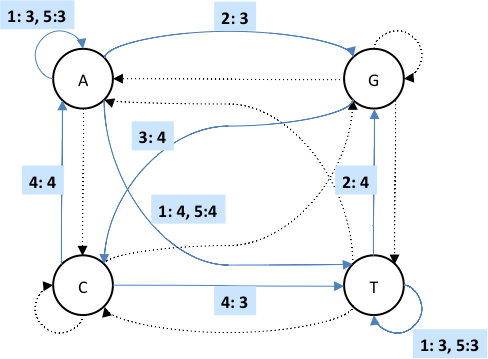
\includegraphics[width=0.45 \textwidth]{fig05/fsm_solution.png}
\end{figure}

%% (b)
\part Use the finite-state machine to find the matching segment pairs and the scores.

\begin{enumerate}
\item d1: TCGGTAA

\begin{solution}[0.5 in]
\begin{verbatim}
q: 1 AT 2    Score: 3    q: 5 AT 6    Score: 3
d: 6 AA 7                d: 6 AA 7
\end{verbatim}
\end{solution}

\item d2: ATAGC

\begin{solution}[1 in]
\begin{verbatim}
q: 1 AT 2    Score: 4    q: 5 AT 6    Score: 4
d: 1 AT 2                d: 1 AT 2

q: 2 TG 3    Score: 3    q: 3 GC 4    Score: 4
d: 3 AG 4                d: 4 GC 5
\end{verbatim}
\end{solution}

\end{enumerate}

\end{parts}

